\documentclass{article}
\usepackage{graphicx} % Inserting graphics (\includegraphics{<graphic>}) https://www.overleaf.com/learn/latex/Inserting_Images
\usepackage{amssymb,amsmath,amsthm} % Math symbols, enviroments and more
\usepackage{xcolor} % Changing text color (\textcolor{<color>}{<text>}) https://www.overleaf.com/learn/latex/Using_colours_in_LaTeX
\usepackage{float} % Provides H specifier for floats
\usepackage[output-decimal-marker=\text{,}, exponent-product=\ensuremath{\cdot}, range-phrase={ - }]{siunitx} % SI units with correct number formatting (\num{<value>}, \si{<unit>}, \SI{<value>}{<unit>})
\usepackage{hyperref} % Hyperlinks (\href{<url>}{<text>}, \url{<url>}) https://www.overleaf.com/learn/latex/Hyperlinks
\usepackage{pgf} % Graphics https://www.overleaf.com/learn/latex/TikZ_package
\usepackage[siunitx, RPvoltages, european]{circuitikz} % Drawing circuits https://www.overleaf.com/learn/latex/CircuiTikz_package
\usepackage{multicol} % Allows merging multiple cells in one table row (\multicolumn{<number of columns>}{<style eg. |c>}{<content>})
\usepackage{multirow} % Merging multiple cells in one table column (\multirow{<number of rows>}{<width eg. * for natural width>}{<content>}
\usepackage{pgfplots} % Data plots https://www.overleaf.com/learn/latex/Pgfplots_package
\pgfplotsset{compat=1.18} 
\usepackage{pdfpages} % Allows inserting a pdf page (\includepdf[pages=<which pages, - for all>]{<filename>})
\usepackage[a4paper, margin=1in]{geometry} % Sets paper size to A4 with content no bigger than 6 by 8 inch https://www.overleaf.com/learn/latex/Page_size_and_margins
\usepgfplotslibrary{polar}
\usepackage{csvsimple} % Creating tables based on CSV's
\usepackage{lscape} % Landscape pages (\begin{landscape})
%%\usetikzlibrary{external} % Caching images
%\tikzexternalize[prefix=tikz/] % Caching images
\usepackage{subfig}  % Multiple figures in a row
\DeclareSIUnit\torr{Torr}
\usepackage{rotating}
\usepackage{pdflscape}
\usetikzlibrary{shapes.geometric, arrows}
\usepackage{listings}

\title{Ion Gauge Controller}
\author{Jakub Jendryka}
\date{22.10.2023}

\begin{document}
\maketitle

\section{Introduction}
This project is a Bayard-Alpert vacuum gauge controller designed to work within the EuroMeasure system.
\subsection{Bayard-Alpert gauge}
Bayard-Alpert gauge is a type of a vacuum gauge that uses gas ionization through electron impact as a way
to measure high vacuums in the range of \SI{1e-3}{Torr} - \SI{1e-10}{Torr} or \SI{1e-1}{\pascal} - \SI{1e-8}{\pascal}.
Electrons are boiled-off from the cathode which is a tungsten filament heated with a current passed through it.
Electrons are then accelerated using a grid at a strong positive potential.
Accelerated electrons going through the vacuum have a chance to struck a residual gas molecule and ionise it.
This, now positively charged, ion is attracted by the anode at a slight negative potential.
Current that flows into the anode due to those ions is therefore proportional to the pressure inside the gauge.

\begin{figure}[H]
	\begin{center}
		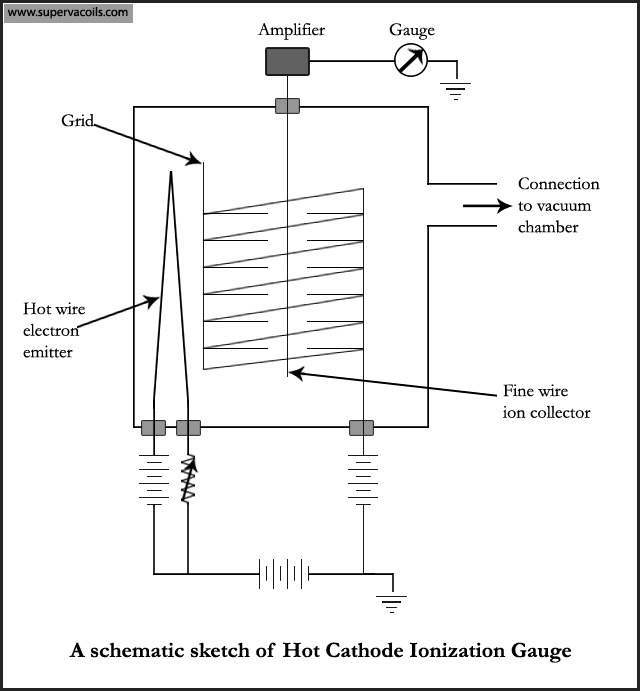
\includegraphics[width=0.5\textwidth]{figures/ion_gauge.jpg}
	\end{center}
	\caption{Hot ionisation vacuum gauge diagram}
	\label{fig:ion_gauge}
	% https://www.supervacoils.com/vacuum-gauges-explained/hot-ionization-gauge/
\end{figure}


\subsection{EuroMeasure}
EuroMeasure is a mechanical, electronic and protocol standard for measurement and control systems.
It is developed at Wrocław University of Science and Technology faculty of Microsystems. This standard defines a module that can be connected with others on a single bus.
It was designed to be compatible with standard Eurocard enclousures as well as to be cheap to manufacture.
Each module consists of one or more PCB's, each taking up one module width. Each PCB can be connected to a backplane using two IDC10 connectors providing power and control signals and can also have an additional debug connector.
Additional connectors and other parts needed for operation can be mounted on the module front panel, which is attached to the PCB's.

\section{Requirements}
From the theory of operation of the vacuum gauge arise several requirements. The controller needs to heat the cathode, polarize all the electrodes in relation to each other and measure currents flowing in and out of the electrodes.
This device is expected to operate with SJ2 vacuum gauge. Gauge parameters per its datasheet are as follows:
\begin{itemize}
	\item Cathode current: \SI{1.5}{\ampere}$\pm$\SI{0.1}{\ampere}
	\item Cathode emission current: \SI{5}{\milli\ampere}
	\item Grid voltage: \SI{200}{\volt}
	\item Anode voltage: \SI{-25}{\volt}
	\item Sensitivity: \SI{16}{\frac{\milli\ampere}{\milli\ampere\cdot\torr}}
	\item Working range: \SIrange{1e-7}{1e-3}{\torr}
\end{itemize}

It is expected that cathode current is adjusted to stabilize electron emission current at the required level.
Using working range, emission current and sensitivity, anode current range can be calculated to be around: \SI{10}{\nano\ampere} - \SI{100}{\micro\ampere}.
Cathode voltage at specified current was measured to be around \SI{8}{\volt}.
In summary the device needs to supply continously adjustable cathode current, polarize the grid and measure grid current, polarize the anode and measure anode current.
It would be beneficial if parameters of the device were adjustable, as most Bayard-Alpert gauges have similar requirements and this would allow to support other models.

As the device is going to be a part of EuroMeasure system it needs to conform to its specification.
It is expected that it will take up one module width, therefore it should consist of one \num{10}$\times$\SI{10}{\centi\meter} PCB with max
component height of \SI{16}{\milli\meter} at the top and \SI{2}{\milli\meter} at the bottom. There are four M3 mounting holes at the corners of the PCB, \SI{5}{\milli\meter} from the edge.
There are three right-angle IDC10 connectors at the back edge of the board. One for power ($\pm$\SI{15}{\volt} and $+$\SI{5}{\volt}), one for data (I2C communication and high voltage lockout) and one for debugging (SWD and UART).
Connector for the vacuum gauge should be mounted to the front panel. The device is expected to operate in standard laboratory conditions.
It should emit as little as possible EMI, and should not backfeed noise onto $\pm$\SI{15}{\volt} power supply rails and should disable hazardous voltages when lockout line is not energized.

\section{Schematic}

Block diagram of the design is presented on the next page. It also serves as top level schematic sheet.
Starting with the gauge it is connected to the controller using a single connector. Each of the electrodes is supplied by a separate switchmode power supply.
Anode and grid power supplies are constant voltage, not controllable power supplies with galvanicly isolated output. This allows for easy current measurement on the low side of the supply.
Cathode supply is programmable constant voltage switchmode supply. Using current measurement data from the grid, microcontroller can modify output voltage to stabilize emission current at required level.
To allow for cathode health monitoring, its voltage as well as current are monitored.
As cathode response is not very fast due to its thermal mass it was decided to use a fully digital control loop, as it will be easier to implement and add cathode safety features that disallow accidental cathode burnout.
Every important parameter is digitized in the ADC block and processed by the microcontroller. Power and interface are connected through the backplane connector.
To minimize backfed noise, voltages suppling power supplies are filtered.

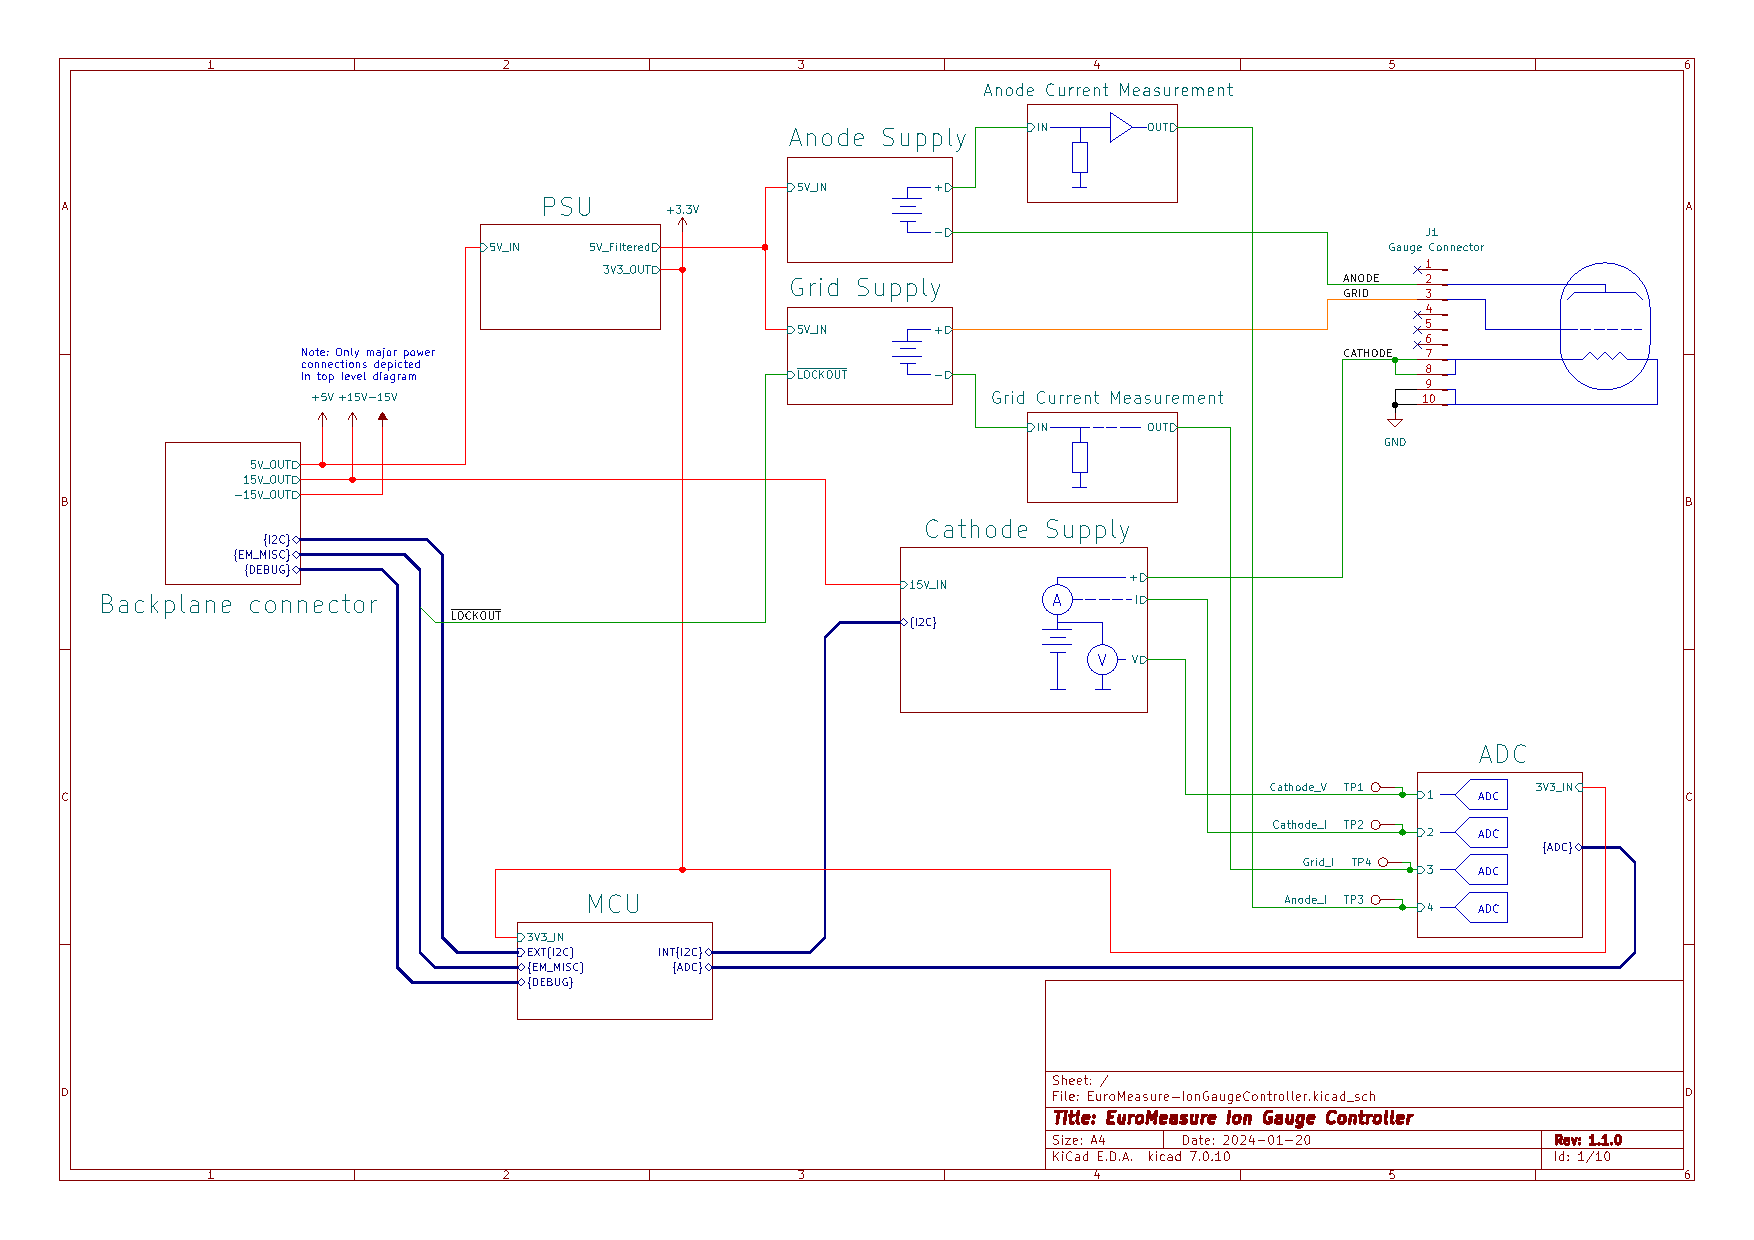
\includepdf[landscape=true, pages=1]{figures/schematic.pdf}



\subsection{Anode supply}
To generate anode voltage SN6507 push-pull transformer driver was selected. It was already tested in a previous project and offered required low-noise operation due to configurable slew rate.
To pair with the driver 750316856 transformer was selected. It offered high enough turn ratio of \num{4.67} (It was decided to set this voltage pretty high to be able to modify output voltage in the future).
Output voltage was calculated using equation \ref{eq:anode_dcdc_voltage}:
\begin{equation}
	V_{out} = 2\cdot V_{in} \cdot n_{ratio}  = 2 \cdot \SI{5}{\volt} \cdot \num{4.67} = \SI{46.7}{\volt}
	\label{eq:anode_dcdc_voltage}
\end{equation}
To not saturate the core, sufficiently high switching voltage is required. Manufacturer specifies transformer "voltage-time" to be \SI{15}{\volt\micro\second}.
Minimum frequency is calculated using equation \ref{eq:transformer_saturation}.
\begin{equation}
	F_{min} = \frac{V_{in}}{VT} = \frac{\SI{5}{\volt}}{\SI{15}{\volt\micro\second}} = \SI{333}{\kilo\hertz}
	\label{eq:transformer_saturation}
\end{equation}
To have sufficient margin operating frequency was set to \SI{500}{\kilo\hertz}. To do this, resistor R16 was set to \SI{22}{\kilo\ohm} in accordance to the specification.
Programmable current limit was set to \SI{500}{\milli\ampere} with R22, and soft start time was set to \SI{3.8}{\milli\second} according to equation \ref{eq:anode_soft_start}.
\begin{equation}
	T_{ss} = \frac{C_{17}}{\SI{275}{\micro\ampere}-\frac{0.6}{R_{17}}} = \SI{3.8}{\milli\second}
	\label{eq:anode_soft_start}
\end{equation}
Undervoltage lockout was set to be around \SI{3.8}{\volt} (eq. \ref{eq:anode_undervoltage}).
\begin{equation}
	U_{UVLO} = \SI{1.5}{\volt} \cdot \left(1+\frac{R_{19}}{R_{15}}\right) = \SI{3.8}{\volt}
	\label{eq:anode_undervoltage}
\end{equation}

Voltage from the transformer is rectified with a full bridge rectifier build using "low-emission" PMEG200G20 diodes. Their low forward voltage and reverse charge limit switching noise.
Voltage is then filtered using capacitors and an inductor. LTSpice simulations show around \SI{-75}{\deci\bel} damping at switching frequency. It is very important to take into account capacitor derating due to DC bias.
To further reduce noise and stabilize voltage level, an adjustable voltage regulator is used.
It's output voltage is set using R22 and R22 according to the equation \ref{eq:anode_output_voltage}. Diodes D12 and D13 are added for IC protection from capacitor discharge, following manufacurer recommendation.
\begin{equation}
	V_{out}= \SI{1.25}{\volt}\cdot\left(1+\frac{R_{22}}{R_{21}}\right) + \SI{50}{\micro\ampere}\cdot R_{22}
	\label{eq:anode_output_voltage}
\end{equation}

\subsection{Anode current measurement}
Anode current measurement is the most critical measurement in the whole device. Due to this extra care must be taken. Transimpedance amplifier configuration was considered, however stability concerns dictated the change to the current configuration.
Anode current is measured using R41 \SI{1}{\kilo\ohm} resistor. This gives voltage of \SI{0.1}{\volt} for full range of \SI{100}{\micro\ampere}. This voltage shift should not influence the measurement significantly as it is only a \SI{0.4}{\%} change.
Due to voltage in the low measurement range being only \SI{10}{\micro\volt} a low offset precision op-amp is needed for amplification of the signal.
OPA2187 was selected as it specifies low offset voltage of \SI{10}{\micro\volt} with drift of only \SI{0.001}{\micro\volt/\kelvin} and bias current of \SI{100}{\pico\ampere}.
It is used to provide a gain of x11 to more fully utilise ADC range. Diode DZ3 is added for ADC protection.

\includepdf[landscape=true, pages=4]{figures/schematic.pdf}
\includepdf[landscape=true, pages=7]{figures/schematic.pdf}

\subsection{Grid supply}
Grid requires the highest of all needed voltages. To generate it, Royer converter topology was selected due to its very low noise. The whole supply is heavily inspired by AN-118 note by Jim Williams.
Resonant Royer converter is a self-oscillating circuit that uses core saturation as means of limiting the oscillation. Due to it's sinusoidal waveforms, no high frequency switching noise is generated.
Main LC tank is created with the transformer primary winding and capacitor C11. Transistors Q1 and Q3 are driven alternately in sync with the LC tank by a transformer feedback winding.
Transformer output is rectified with a full bridge rectifier and further filtered. The circuit has two feedback paths, one AC and one DC. DC path is used to accurately control the output voltage, while AC improves transient response by bypassing the output filter.
The resonant converter output amplitude is controlled by controlling current going to the converter with Q2. Output voltage is settable by changing the resistive divider in the DC feedback path (R13 and R14).

\subsection{Grid current measurement}
Due to low precision needed, relatively high current and output voltage, measuring the grid current by means of a simple resistor is sufficient. Voltage from the resistor is filtered and limited by DZ3 diode to protect the ADC.
With two \SI{100}{\ohm} resistors, the circuit has a sensitivity of \SI{0.2}{\volt/\milli\ampere} which gives \SI{1}{\volt} for nominal emission current, while ADC range is \SI{1.2}{\volt}.

\includepdf[landscape=true, pages=3]{figures/schematic.pdf}
\includepdf[landscape=true, pages=8]{figures/schematic.pdf}

\subsection{Cathode supply}
Cathode supply has to provide the most wattage in comparison to anode and grid supplies. Its parameters are also least crucial as it is only used to heat the cathode and it doesn't need galvanic isolation for precise current measurement.
It however needs to be controllable to stabilize the emission current, but this control loop doesn't have to work at high frequency.
It was decided to use a modern integrated DCDC converter IC. TPS55289 was selected. It allows to control the output voltage from I2C bus without complicated circuitry. It also has undervoltage protection, current monitoring, overcurrent protection and more.
The IC is implemented according to the datasheet and using spreadsheet provided by the manufacturer. To provide the required power it was decided to use the \SI{15}{\volt} rail. To not backfeed noise onto this rail, a filer is used. Capacitors C27 and C37 were selected to have very low ESR to limit ripple.
Undervoltage lockout was set using R27 and R28 to \SI{13.8}{\volt} according to the equation \ref{eq:cathode_uvlo}.
\begin{equation}
	U_{UVLO} = \SI{1.23}{\volt}\cdot\left(1+\frac{R_{27}}{R_{28}}\right) = \SI{13.8}{\volt}
	\label{eq:cathode_uvlo}
\end{equation}
In case of too much switching noise, additional snubber circuits are planned however not populated right now. Frequency dithering is disabled, however to enable it R26 needs to be replaced with a capacitor. Example value in \SI{10}{\nano\farad}.
External feedback is also not connected by default as it most probably won't be neccessery. To enable it R34 resistor needs to be populated and it needs to be enabled in IC configuration registers. Address of the IC is set to 0x75 by connecting MODE pin to ground.
Switching frequency is set using R29 and its value is calculated using equation \ref{eq:cathode_freq}.
\begin{equation}
	f = \frac{1000}{0.05*R_{29}+35} = \SI{420}{\kilo\hertz}
	\label{eq:cathode_freq}
\end{equation}
To reduce heating of the IC, \SI{5}{\volt} is supplied to it externaly, instead of relying on internal voltage regulator. To do this EXTVCC pin had to be connected to logic low, and 5V needed to be connected to VCC.
Current measurement functionality of the IC is also utilised. Current is measured using a shunt resistor R32. A small value of \SI{20}{\milli\ohm} was selected to limit the voltage drop to \SI{30}{\milli\volt}.
Voltage drop on the resistor is amplified in the IC by a factor of 20 and output on pin CDC. Output voltage is also measured by the ADC to control whether the converter is operating correctly.
\includepdf[landscape=true, pages=5]{figures/schematic.pdf}

\subsection{ADC}
To measure all required voltages a dedicated analog to digital converter is used. There are 4 signals that need to be digitized: anode current, grid current, cathode current and cathode voltage.
ADS131M04 was selected as it offers 4 simultaneous channels, precision required for anode current measurement without ranging and was already used in other module of EuroMeasure system.
Its a 24 bit sigma delta ADC with integrated digital averaging and filtering, high precision voltage reference and programmable gain amplifier.
It communicates with the microcontroller using \SI{3.3}{\volt} SPI interface and two additional signals: DRDY(data ready) and RESET.
It required an external clock source. It is implemented using a \SI{8.192}{\mega\hertz} oscillator, as specified in the datasheet.
It is powered from \SI{3.3}{\volt} rail with additional filtering.
All signals connected to the IC are already in the correct $\pm$\SI{1.2}{\volt} range.

\includepdf[landscape=true, pages=6]{figures/schematic.pdf}

\subsection{Microcontroller}
An STM32G0 is used as a microcontroller on this board. It is used in almost all other EuroMeasure modules. Its implementation is also standard between them. It's clocked with a \SI{16}{\mega\hertz} oscillator.
It is powered using \SI{3.3}{\volt} rail generated using a voltage regulator. It's connected to all digital interfaces on the board: DCDC's I2C, ADC's SPI and EuroMeasure signals connected from backplane.
It is also connected to a debug connector with UART and SWD for programming and debuging. For status indication one red LED and one programmable RGB led are used.
All of the digital interfaces use \SI{3.3}{\volt} logic so no voltage translation is needed. To select adress in the EuroMeasure system a DIP switch is used or, alternatively solderable jumpers.
\includepdf[landscape=true, pages=2]{figures/schematic.pdf}
\includepdf[landscape=true, pages=10]{figures/schematic.pdf}
\includepdf[landscape=true, pages=9]{figures/schematic.pdf}

\section{Layout}
The controller is layed out on a single $100\times100\si{\milli\meter}$ two layer PCB.
Almost all components needed to be placed on the top side of the PCB due to height limitations.
Mounting hole as well as backplane connector positions are specified by the EuroMeasure standard.
Microcontroller as well as PSU sections are used on other boards therefore their layout is a copy of already existing designs and is placed on the right side of the board, near the backplane connection.
The most noise sensitive measurement is that of anode current so this circuit is placed further from potential noise emitting sections such as cathode power supply.
To also limit the emissions, all high current loops in the DCDC converters are routed as small as possible and a ground plane is used on the bottom layer with via stitching used where it is not continous.
Via stiching was also used around the anode power supply to make sure that none of the currents from other converters go near it.
Some components on the board, such as power transistors, voltage regulators and cathode DCDC converter IC produce a lot of heat, therefore additional copper pours are placed on their heat dissapating pins.
To increase separation of copper from the high voltage nets in grid power supply a keep-out zone was created where no copper pour will be generated.


\section{Software}
Main factor driving the software design was the need to conform to the EuroMeasure standard. Within this standard each module has an address and a set of commands that it can execute.
Each command can have multiple arguments and it also can return multiple values. Each module also must implement a basic set of commands used for automatic functionality discovery. When interrogated is should describe all commands it implements.
Commands are sent through an I2C interface in a binary format. Most of the EuroMeasure interface is implemented in a dedicated library, so functionality such as standard commands, I2C interface handling and command registration doesn't need to be reimplemented.
Additional commands that need to be implemented are:
\begin{itemize}
	\item Switching cathode heating ON/OFF
	\item Reading the pressure
	\item Reading diagnostic values, such as emission current and heating power
\end{itemize}
Apart from listening to the commands, this module has to continously execute a control loop for stabilizing the emission current and monitor the safety of the cathode which should be disabled in case of too high pressure.
Main flow of the program is represented in figure \ref{fig:diagram}, however due to heavy use of interrupts,
it doesn't adequately describe the full operation. To do that aditional diagrams are needed presented in figure \ref{fig:i2c_diagram} and \ref{fig:adc_diagram} which describe I2C interupt handler and ADC interupt handler accordingly.

\tikzstyle{startstop} = [rectangle, rounded corners, minimum width=2cm, minimum height=1cm,text centered, draw=black, fill=red!30]
\tikzstyle{io} = [trapezium, trapezium stretches=true, trapezium left angle=70, trapezium right angle=110, minimum width=2cm, minimum height=1cm, text centered, draw=black, fill=blue!30]
\tikzstyle{process} = [rectangle, minimum width=2cm, minimum height=1cm, text centered, draw=black, fill=orange!30]
\tikzstyle{decision} = [diamond, aspect=2, minimum width=2cm, minimum height=1cm, text centered, draw=black, fill=green!30]
\tikzstyle{arrow} = [thick,->,>=stealth]
\tikzstyle{line} = [thick, >=stealth]
\begin{figure}[H]
	\centering
	\begin{tikzpicture}[node distance=2cm]
		\node (start)[startstop]{Start};
		\node (init)[process, below of=start]{Initialize ADC and DCDC};
		\node (cathode_on)[decision, below of=init]{Is cathode on?};
		\node (wait)[process, left of=cathode_on, xshift=-2cm]{Wait};
		\node (pressure_ok)[decision, below of=cathode_on]{Is pressure ok?};
		\node (disable)[io, right of=pressure_ok, xshift=2cm]{Disable cathode};
		\node (adj_v)[io, below of=pressure_ok]{Adjust cathode voltage};

		\draw [arrow](start)--(init);
		\draw [arrow](init)--(cathode_on);
		\draw [arrow](cathode_on)--node[anchor=south]{No}(wait);
		\draw [arrow](cathode_on)--node[anchor=west]{Yes}(pressure_ok);
		\draw [arrow](pressure_ok)--node[anchor=south]{No}(disable);
		\draw [arrow](pressure_ok)--node[anchor=west]{Yes}(adj_v);
		\draw [line](wait)--++(0, 1.25cm)-|(cathode_on);
		\draw [line](disable)--++(0, 3.25cm)-|(cathode_on);
		\draw [line](adj_v)--++(7cm, 0)--++(0, 5.25cm)-|(cathode_on);
	\end{tikzpicture}
	\caption{Main flow diagram}
	\label{fig:diagram}
\end{figure}
\begin{figure}[H]
	\centering
	\begin{tikzpicture}[node distance=2cm]
		\node (start)[startstop]{I2C interrupt};
		\node (receive)[io, below of=start]{Receive I2C message};
		\node (select)[decision, below of=receive]{Select command handler};
		\node (enable)[process, below of=select, xshift=3cm]{Enable cathode};
		\node (disable)[process, below of=select, yshift=-2cm, xshift=3cm]{Disable cathode};
		\node (measure)[io, below of=select, yshift=-4cm, xshift=3cm]{Return last pressure};
		\node (dotdotdot)[process, below of=select, yshift=-6cm, xshift=3cm]{...};



		\draw [arrow](start)--(receive);
		\draw [arrow](receive)--(select);
		\draw [arrow](select)|-(enable);
		\draw [arrow](select)|-(disable);
		\draw [arrow](select)|-(measure);
		\draw [arrow](select)|-(dotdotdot);
		%\draw [arrow](cathode_on)--node[anchor=west]{Yes}(pressure_ok);
		%\draw [arrow](pressure_ok)--node[anchor=south]{No}(disable);
		%\draw [arrow](pressure_ok)--node[anchor=west]{Yes}(adj_v);
		%\draw [line](wait)--++(0, 1.25cm)-|(cathode_on);
		%\draw [line](disable)--++(0, 3.25cm)-|(cathode_on);
		%\draw [line](adj_v)--++(7cm, 0)--++(0, 5.25cm)-|(cathode_on);
	\end{tikzpicture}
	\caption{I2C interrupt handler diagram}
	\label{fig:i2c_diagram}
\end{figure}
\begin{figure}[H]
	\centering
	\begin{tikzpicture}[node distance=2cm]
		\node (start)[startstop]{DRDY low interrupt};
		\node (transaction)[io, below of=start]{Get values from ADC};
		\node (parse)[process, below of=transaction]{Calculate currents and pressure};
		\node (store)[process, below of=parse]{Store values};

		\draw [arrow](start)--(transaction);
		\draw [arrow](transaction)--(parse);
		\draw [arrow](parse)--(store);

	\end{tikzpicture}
	\caption{ADC interrupt handler diagram}
	\label{fig:adc_diagram}
\end{figure}

\subsection{Code snippets}
\subsection{ADC data acquisition}
Listing \ref{lst:adc} shows code responsible for acquiring samples from the ADC. It is called within interrupt handler subroutine for DRDY pin change. To download the data from ADC an SPI transaction is performed.
ADC is configured to communicate in 24-bit words, therefore each word takes up 3 bytes. ADC talks with standardized transactions,
every frame send by the ADC consists of response from last command (if no command was issued it returns STATUS register contents), data from each of 4 channels and a CRC code.
Endianess of ADC data doesn't match MCU endianess therefore bytes need to be swaped. Special consideration also needs to be taken as data is supplied in two's complement format and in 24-bit format, whereas native word size for the MCU is 32-bit.
SPI_transaction function is written to handle bidirectional data transfer.
\lstinputlisting[language=C, tabsize=2, showspaces=false, xleftmargin=0cm, frame=tblr, breaklines=true, caption=Code acquiring data from ADC, label=lst:adc]{code/adc.c}



\end{document}
